\documentclass[12pt]{article}
\usepackage[T1]{fontenc}
\usepackage[latin9]{inputenc}
\usepackage{geometry}
\geometry{verbose,bmargin=1.25in,lmargin=1.2in,rmargin=1.2in}
\usepackage{color}
\usepackage{float}
\usepackage{amsmath}
\usepackage{amsthm}
\usepackage{amssymb}
\usepackage{graphicx}
\usepackage{setspace}
\usepackage[authoryear]{natbib}
\onehalfspacing
\usepackage[unicode=true,
 bookmarks=false,
 breaklinks=true,pdfborder={0 0 1},backref=section,colorlinks=true]
 {hyperref}

\makeatletter
\makeatother

\begin{document}
\title{Hamlet \thanks{I thank Muse for valuable comments. All errors are, of course, my
own.}}
\author{William Shakespeare\thanks{Email: bill@globe.com }\\
The Globe Theatre }
\maketitle
\begin{abstract}
This play tells the revenge Prince Hamlet is called to wreak upon
his uncle, Claudius, by the ghost of Hamlet's father, King Hamlet.
\end{abstract}

\section{Introduction}

\section{Data}

\section{Estimation Methods}

Hamlet's love for Ophelia can be described by the following equations:

\begin{align}
x & =16\sin^{3}\left(t\right)\label{eq:love}\\
y & =13\cos\left(t\right)-5\cos\left(2t\right)-2\cos\left(3t\right)-\cos\left(4t\right)\nonumber 
\end{align}

\pagebreak{}

\section{Results}

Plotting \eqref{eq:love} $\Rightarrow$
\begin{figure}[H]
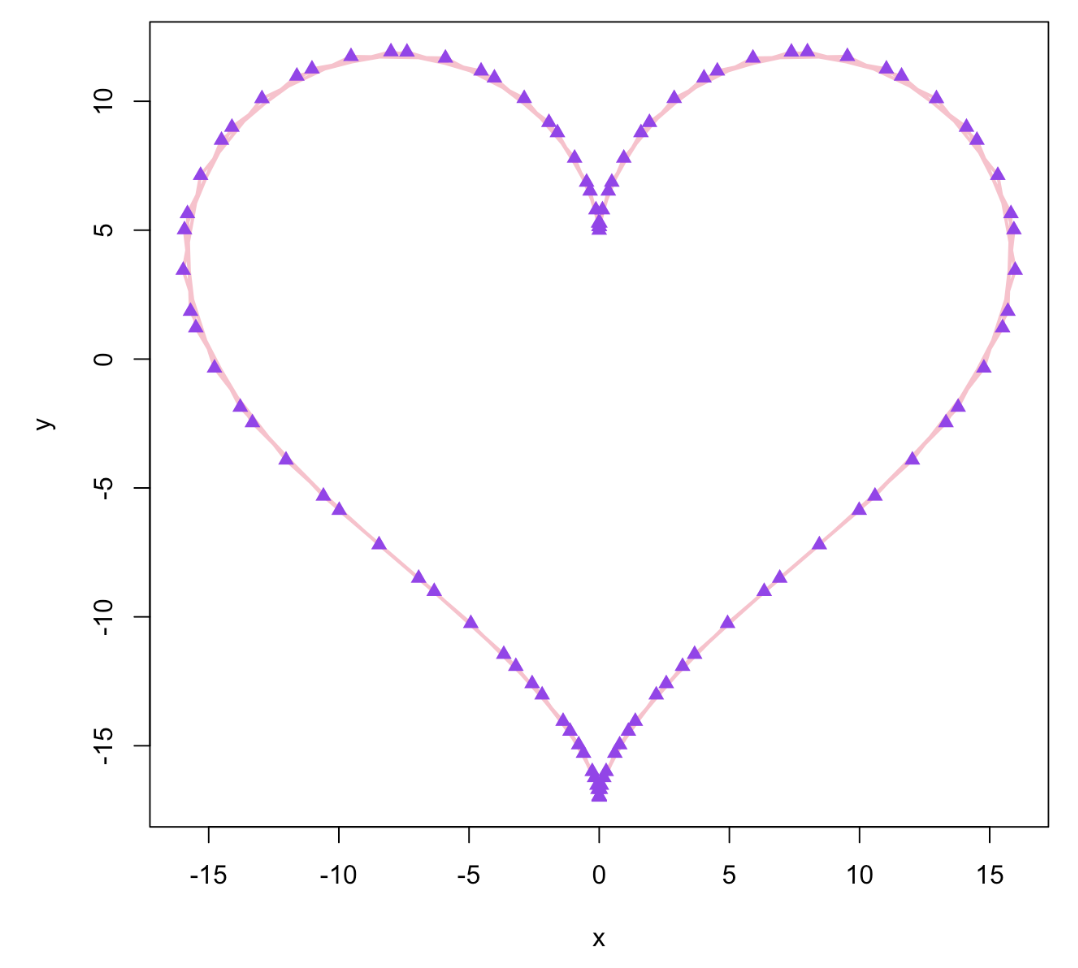
\includegraphics[scale=0.5]{love}

\caption{Hamlet's love for Ophelia}

\end{figure}


\section{Conclusion}
\end{document}
